\section{s-Weighting crosscheck}
\label{app:sWeight}

In order to cross-check out result we applied also an s-Fit technique \cite{Xie:2009rka}. And in this section we compare results on $J/\psi$ data.
This technique which does not need angular PDF for background components as they are statistically subtracted, based
on the invariant the mass projection. In the case of uniform efficiency, the negative log-likelihood has form
\begin{equation}
-\ln\mathcal{L}=-\sum_i w_i P(\cos\theta_{\ell,\Lambda}^i),
\end{equation}
where $w_i$ is signal sWeight for given event and $P(\cos\theta_j^i)$ is signal PDF given by
eqs.~\ref{eq:afbLTh} and \ref{eq:afbBTh} respectively. While using sFit technique allows not to
worry about parametrisation of background, it also has some drawbacks and therefore is not used as default procedure for the measurement.
First of all it underestimates uncertainties and requires a scaleing of the log-likelihood to get correct ones.
Furthermore it's not trivial to implement in the procedure to get errors using the Feldman Cousins techinque,
because it requires the simulation of a background, which needs to be parameterised.

The mass model used to calculate the s-Weights is the same used for the branching ratio analysis (see \ref{fitDescr}).
In fig \ref{fig:sWjpsi} are shown fits of s-Weighted angular distributions for resonant events with full statistics.
The fit model used for the angular distributions is the same used for the rare channel analysis but the
efficiency is taken from resonant MC events instead of rare.

\begin{figure}[h]
\centering
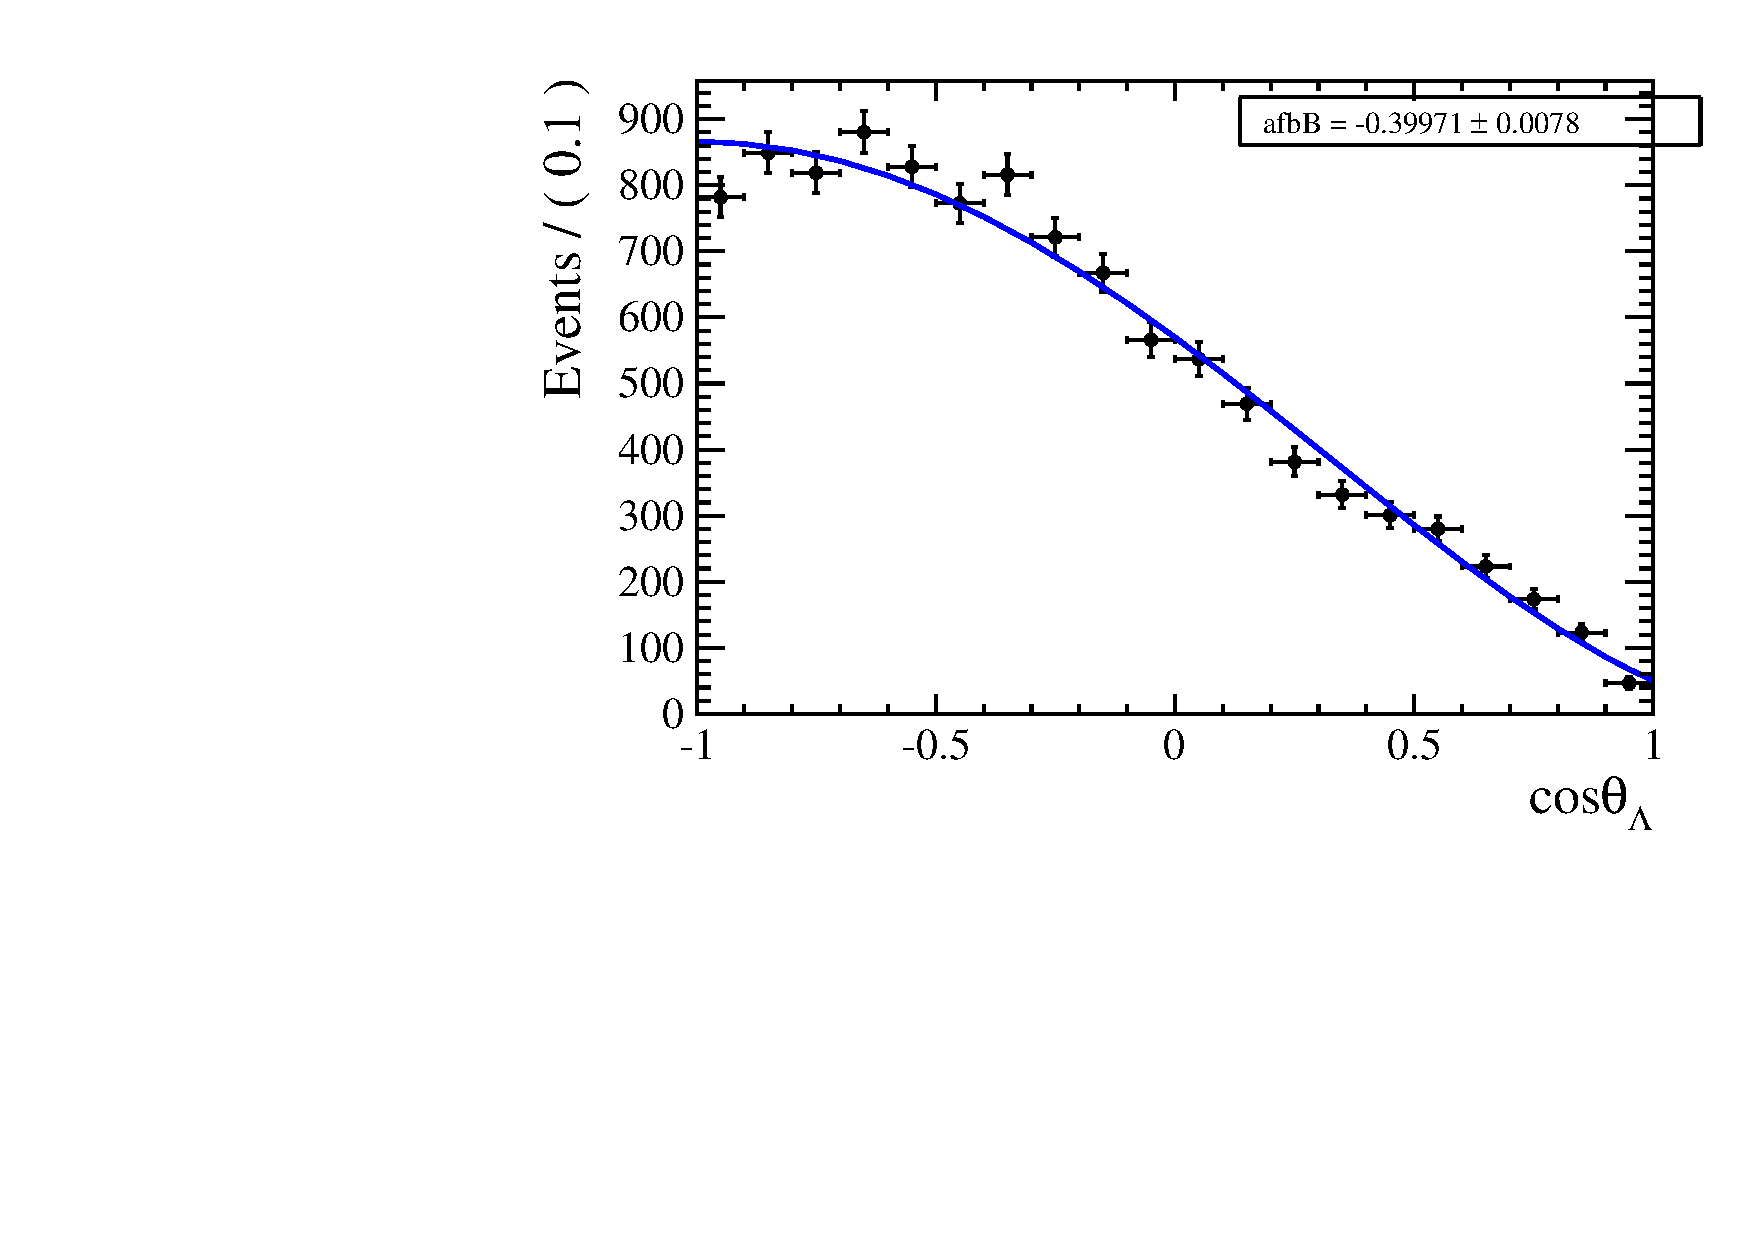
\includegraphics[width=0.4\textwidth]{Lmumu/figs/AfbB_DD_jpsi_sW.pdf}
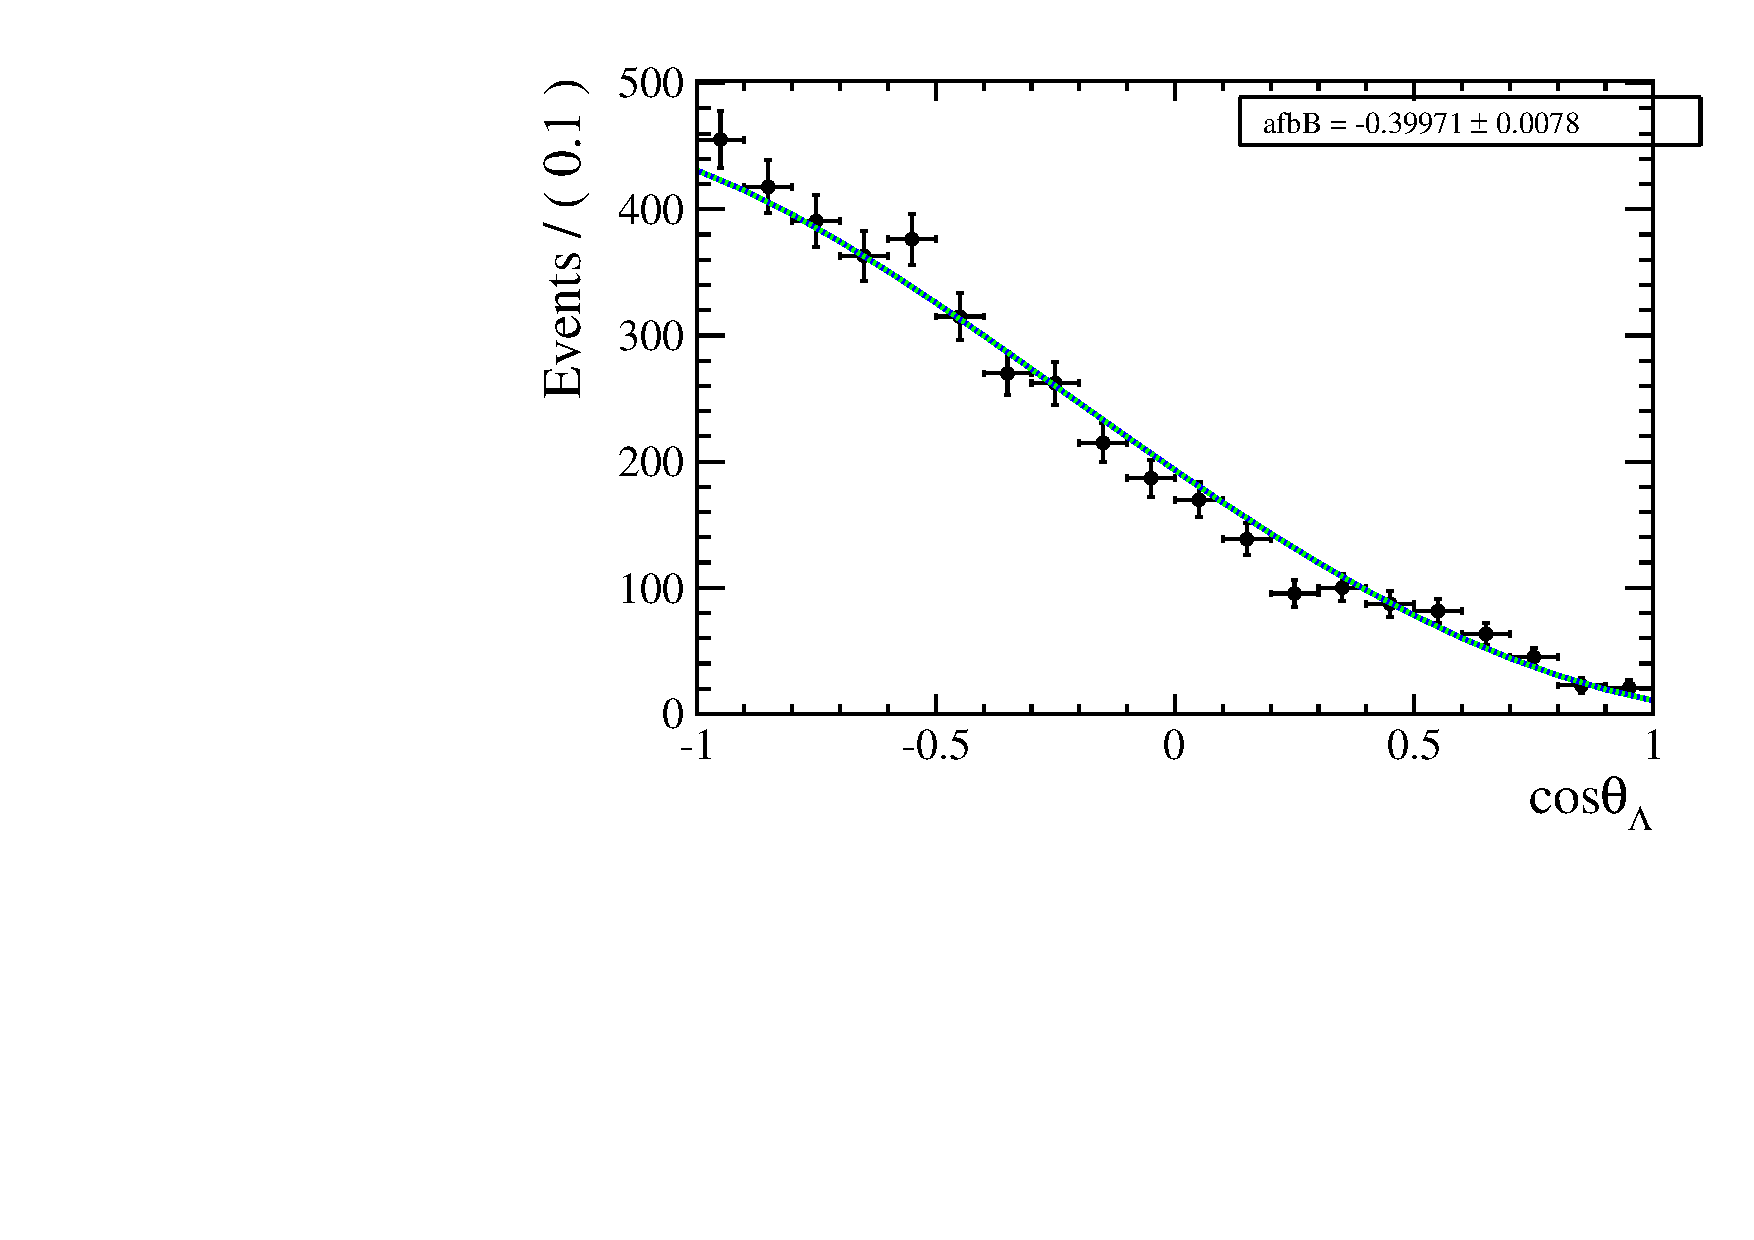
\includegraphics[width=0.4\textwidth]{Lmumu/figs/AfbB_LL_jpsi_sW.pdf} \\
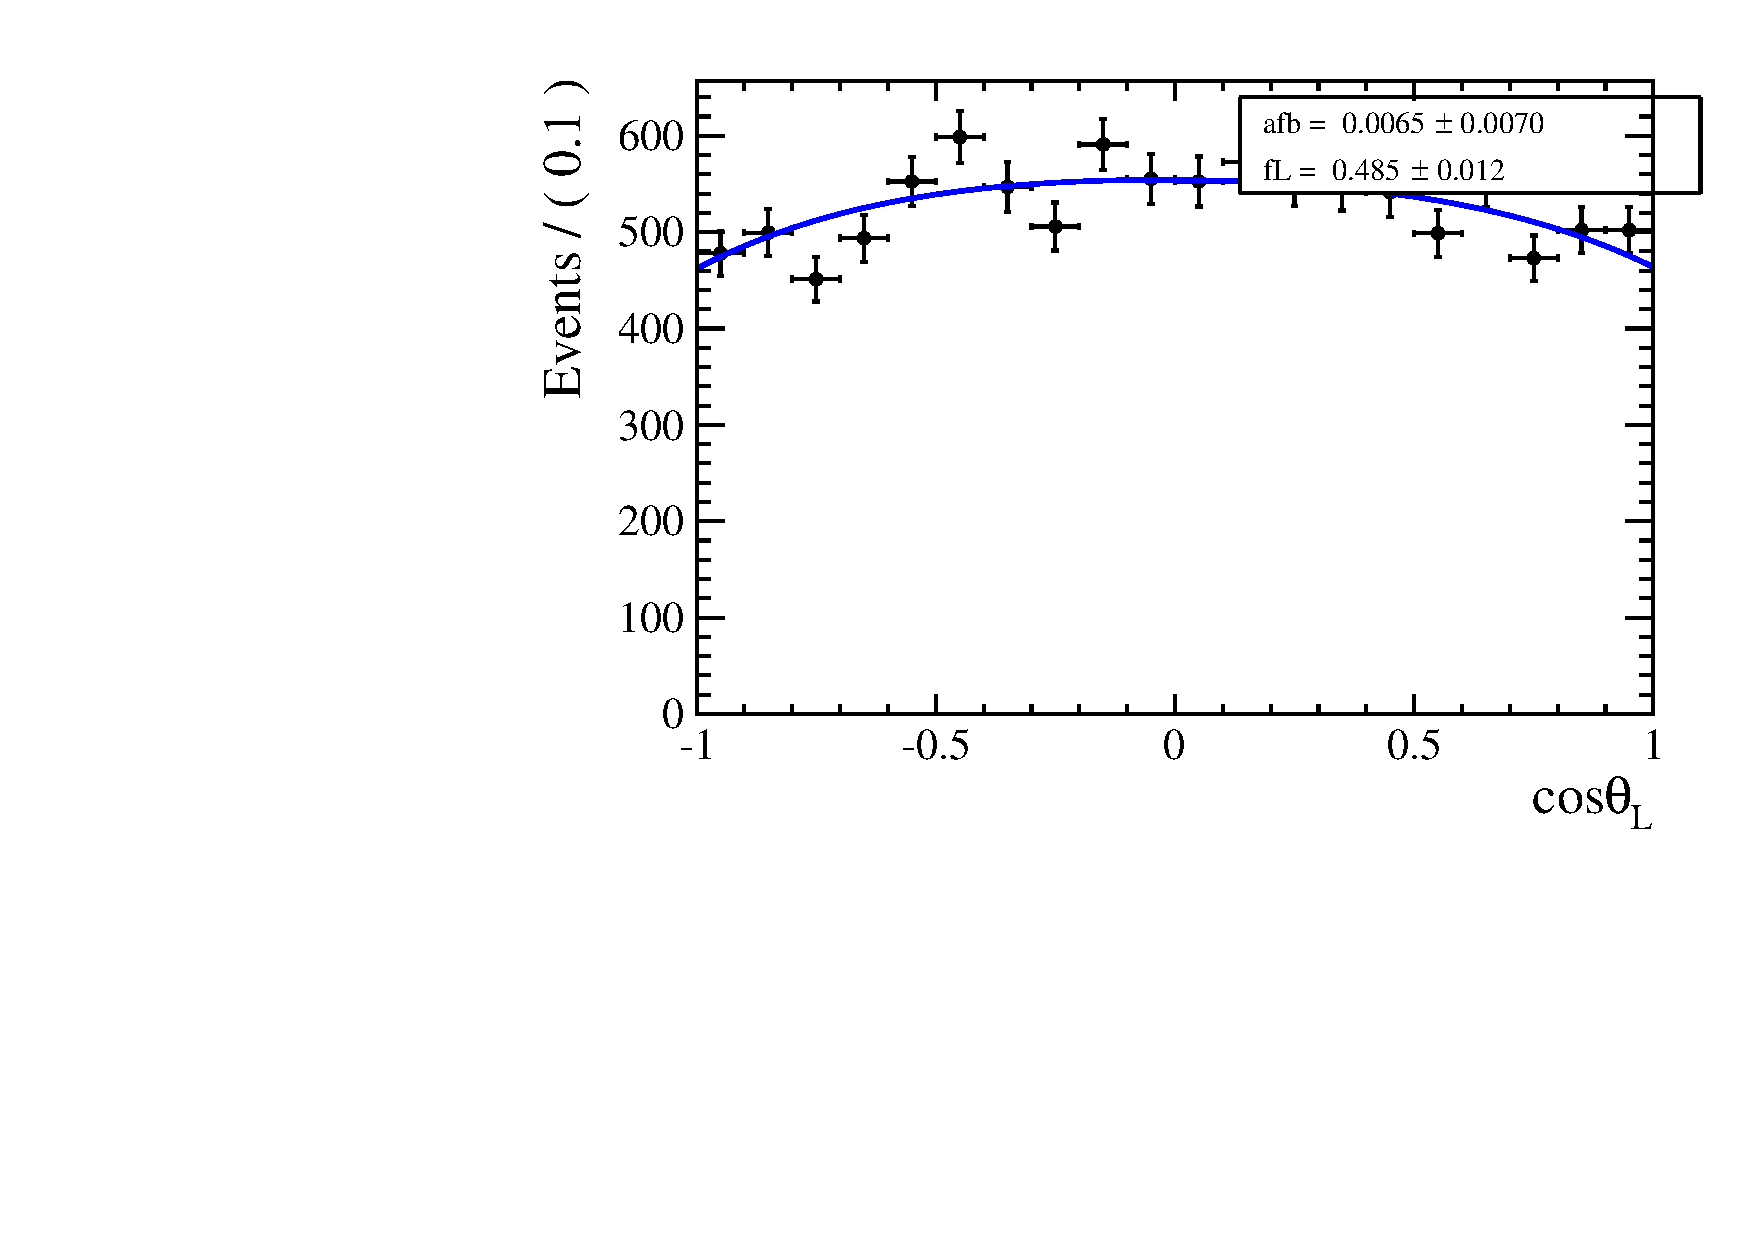
\includegraphics[width=0.4\textwidth]{Lmumu/figs/Afb_DD_jpsi_sW.pdf}
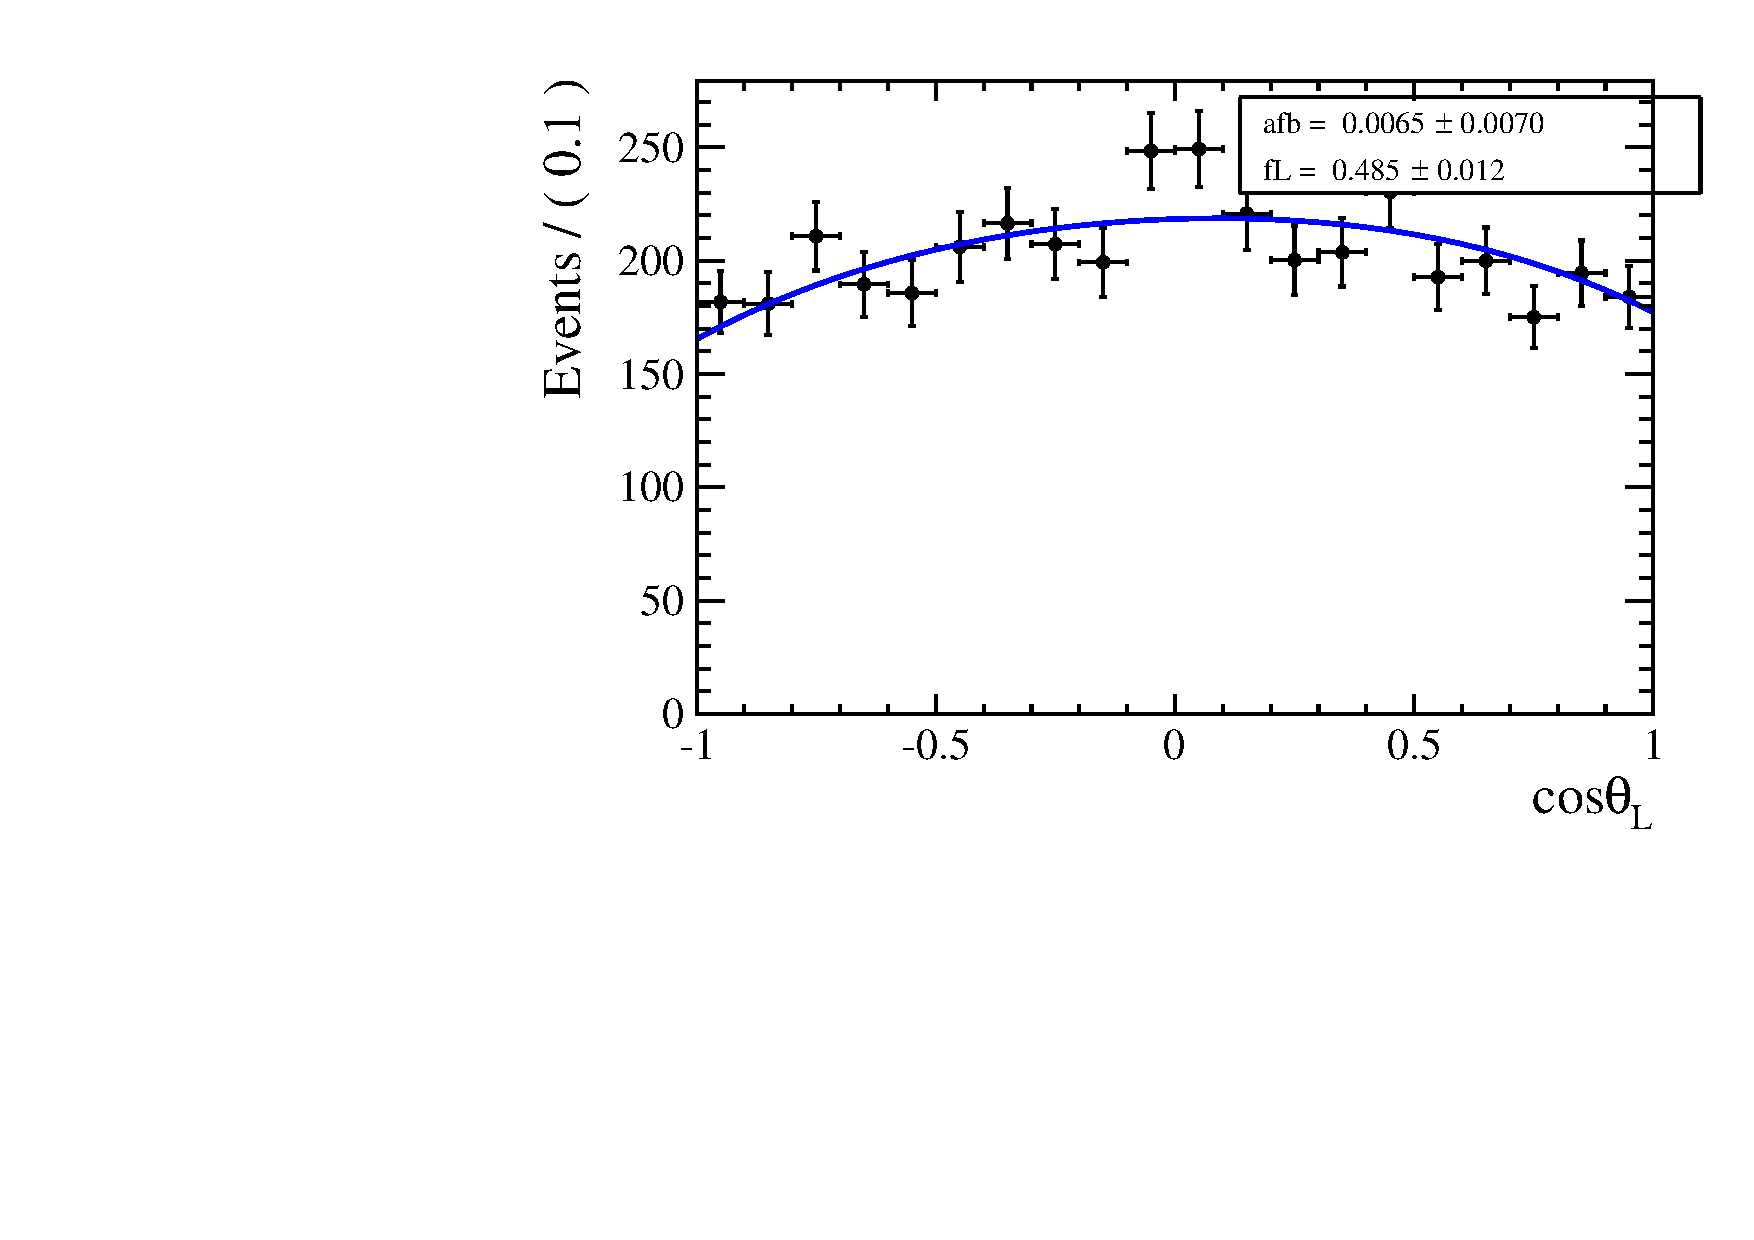
\includegraphics[width=0.4\textwidth]{Lmumu/figs/Afb_LL_jpsi_sW.pdf}
\caption{sWeighted and fitted $\cos\theta_\ell$ (up) and $\cos\theta_\Lambda$ distributions for $\jpsi\Lambda$ events. For down-down (left) and long-long (right) events.  }
\label{fig:sWjpsi}
\end{figure}

Systematics due to the mass modelling in the s-Weighting and the background parameterisation are estimated to be $\sim 0.015$ for all three observables.
Therefore results using the s-Weighting techinique are compatible with the fitting including a background component.
